\documentclass{article}

\author{Author: Jeremy Greenburg \\ Mentor: Dr. Alton Coalter \\ Second Reader: Joshua Guerin}
\title{The God Core \\ A Science Fiction Video Game Developed in C++}

% For importint code and text files
\usepackage{listings}
% For enumerating the Table of Contents
\usepackage{enumitem}
% Incase I need pictures
\usepackage{graphicx}

%Mathematics Galore
\usepackage{amsmath}
\usepackage{amsfonts}
\usepackage{amssymb}
\usepackage{gensymb}

\usepackage{fullpage}

% Subsection numbering
\setcounter{secnumdepth}{3}

% Only Subsections in Table of Contents
\setcounter{tocdepth}{2}

\begin{document}
\maketitle
\pagebreak

\tableofcontents

\pagebreak

\section{Preamble}

\section{Setting}

\section{Programming}

\subsection{The Language}

\subsection{OpenGL}

\subsection{SOIL}

\subsection{FMOD}

\subsection{Classes}

Of the two years of my project, I have constructed \textbf{\textit{CLASSNUM}} classes, across \textbf{\textit{2CLASSNUM}} files. I will describe the classes and there methods here in brief, but the complete files can be found in Appendix 4.1 for your viewing pleasure.

\subsubsection{CameraControl}
The CameraControl class is designed to control and manipulate the player's perspective as they navigate through the game. It contains two ordered triples of floating point numbers: The xyz location of the player, and the rotation along the x axis (looking left/right), the y axis (up/down), and the z axis (barrel roll). It also contains two additional floating point values the, movement speed and the turning speed. 

The CameraControl class contains four methods for rotating the camera, lookUp and lookDown which affect the y rotation, as well as lookLeft and lookRight which affect the x rotation.

There are six movement methods, moveForward and moveBackward are designed to move the camera forward and backwards in respect to where the player is looking currently. This proved quite frustrating to find and I had to ask many math majors for their input until Robert Deyoso was able to help me pin down a formula. These functions adjust the the x and  z coordinates as follows:

z := z $\pm$ moveSpeed * cos(radian(x\_angle))

x := x $\mp$ moveSpeed * sin(radian(x\_angle))

strafeLeft and strafeRight, again, move the camera directly left and directly right according to where the camera is looking. The formula is similar to the above, except the angle is increased or decreased by 90$\degree$.

moveUp and moveDown were the easiest functions to derive, as up and down are independent of the direction the camera is facing, so it is simply increasing and decreasing the y value respectively. 

invertCam increases the z angle by 180$\degree$ to flip the world upside down.
resetCam resets the 3-tuples to their default values (0, 0, -1) for the position and (0, 0, 0) for the angles.

While those functions work to modify the values within the class, Display is the method that actually moves and rotates the camera within the world. It calls glRotate three times to rotate the camera along the respective axis, and then calls glTranslate to move the camera into the correct position.

\subsubsection{HeadsUpDisplay}

The HeadsUpDisplay class is a complex class that overlays a display to present information or display aesthetics such as the helmet's bounds to the player. The class contains four constant integers to designate the boundaries of the screen (bottom, top, left right), as well as two more integers dimTime and darkTime to control the length of the dim and dark functions. There are three strings held by the class, currentAlert dictates information that will be printed to the center of the screen, currentText is what the user is typing, and currentInput is what the user has entered as input into the developer console (for more information, see the next section). The developer console dev, as well as a TextEngine helmet, also reside in this class.

DisplayHud is the activation method, it calls prepare2D, drawHUD, and prepare3D. This is called in the main function every frame unless the player is in a screen. 

prepare2D prepares openGL for rendering 2D images (the HUD is the last item that is drawn to the screen every frame, therefore nothing can cover it) by disabling everything related to the depth buffer and projecting everything onto a matrix that is orthogonal to the screen bounds.

\subsubsection{Rectangle} For collision purposes, when a Rectangle is created it calculates the Plane equation of the rectangle (Form $ax + by + cz + d = 0$).

This equation is calculated using the first three corners of the rectangle (Calling them A, B, and C) as follows:

\noindent
$
\vec{AB} = \left| \begin{array}{c}
	Bx - Ax \\
	By - Ay \\
	Bz - Az
 \end{array} \right|
\vec{AC} = \left| \begin{array}{c}
	Cx - Ax \\
	Cy - Ay \\
	Cz - Az
 \end{array} \right| \\
a = \vec{AB}_2 * \vec{AC}_3 - \vec{AB}_3 * \vec{AC}_2 \\
b = \vec{AB}_3 * \vec{AC}_1 - \vec{AB}_1 * \vec{AC}_3 \\
c = \vec{AB}_1 * \vec{AC}_2 - \vec{AB}_2 * \vec{AC}_1 \\
d = aAx + bAy + cAz
$

We can also derive the norm of the plane using the equation $\sqrt{a^2 + b^2 + c^2}$

\subsubsection{CollisionEngine}
This determines when the player has collided with an object in the world. There are two types of collisions: player-object collisions and player-wall collisions.

Player object collisions are simple to detect, as both the player and the object can be placed within imaginary "bounding spheres" that extend around the player and object. Collision can be detected with this formula:
$\sqrt{(x_2 - x_1) + (y_2 - y_1) + (z_2 - z_1)} < r_2 + r_1$
If the distance between the two spheres is less than the sum of the radii of the two spheres, the they must be colliding.

Player-wall collisions were much harder to reconcile. Because walls tend to be long and thin, you can't simply place one within a bounding sphere, the resulting sphere would simply be too massive.

To rectify that, the collision is split into two phases: broad and narrow.

In the broad phase, we use the plane equation $ax + by + cz + d$ that is derived in the Rectangle section. We use the formula $\frac{ax + by + cz + d}{\sqrt{a^2 + b^2 + c^2}}$, where x, y, and z are the player's x, y, and z coordinates. If the resulting value is less than the radius of the player's bounding sphere, the player has hit that plane and we move onto the narrow phase.

In the narrow phase, each wall is aligned on an axis: x, y, or z. We simply take the largest and smallest values of the coordinates on that axis (for instance, if the wall is x aligned, we take the largest and smallest x value). If the sphere is in between the two values, the player has hit the wall. Otherwise, they hit the plane but not the wall.

\subsubsection{Console}

\subsubsection{MusicManager}

\subsubsection{TextEngine}

\subsubsection{SaveManager}

\subsubsection{Keyboard}

\subsubsection{Rectangle and Triangle}

\subsection{Problems and Frustrations}

\section{Appendices}

\subsection{Source Code}

\subsubsection{main.cpp}
	\lstinputlisting[
				basicstyle=\ttfamily \small,
				numbers=left,
				breaklines=true,
 				linerange={1-1000},
 				firstnumber = 1]{../main.cpp}
 				
\subsubsection{CameraControl.h}
	\lstinputlisting[
					basicstyle=\ttfamily \small,
					numbers=left,
					breaklines=true,
					linerange={1-1000},
					firstnumber = 1]{../CameraControl.h}

\subsubsection{CameraControl.cpp}
	\lstinputlisting[
					basicstyle=\ttfamily \small,
					numbers=left,
					breaklines=true,
					linerange={1-1000},
					firstnumber = 1]{../CameraControl.cpp}
					
\subsubsection{CollisionEngine.h}
	\lstinputlisting[
					basicstyle=\ttfamily \small,
					numbers=left,
					breaklines=true,
					linerange={1-1000},
					firstnumber = 1]{../CollisionEngine.h}
					
\subsubsection{CollisionEngine.cpp}
	\lstinputlisting[
					basicstyle=\ttfamily \small,
					numbers=left,
					breaklines=true,
					linerange={1-1000},
					firstnumber = 1]{../CollisionEngine.cpp}
					
\subsubsection{Console.h}
	\lstinputlisting[
					basicstyle=\ttfamily \small,
					numbers=left,
					breaklines=true,
					linerange={1-1000},
					firstnumber = 1]{../Console.h}
					
\subsubsection{Console.cpp}
	\lstinputlisting[
					basicstyle=\ttfamily \small,
					numbers=left,
					breaklines=true,
					linerange={1-1000},
					firstnumber = 1]{../Console.cpp}
					
\subsubsection{Cylinder.h}
	\lstinputlisting[
					basicstyle=\ttfamily \small,
					numbers=left,
					breaklines=true,
					linerange={1-1000},
					firstnumber = 1]{../Cylinder.h}
					
\subsubsection{Cylinder.cpp}
	\lstinputlisting[
					basicstyle=\ttfamily \small,
					numbers=left,
					breaklines=true,
					linerange={1-1000},
					firstnumber = 1]{../Cylinder.cpp}
					
\subsubsection{Door.h}
	\lstinputlisting[
					basicstyle=\ttfamily \small,
					numbers=left,
					breaklines=true,
					linerange={1-1000},
					firstnumber = 1]{../Door.h}

\subsubsection{Door.cpp}
	\lstinputlisting[
					basicstyle=\ttfamily \small,
					numbers=left,
					breaklines=true,
					linerange={1-1000},
					firstnumber = 1]{../Door.cpp}
 				
\subsubsection{GameManager.h}
	\lstinputlisting[
					basicstyle=\ttfamily \small,
					numbers=left,
					breaklines=true,
	 				linerange={1-1000},
	 				firstnumber = 1]{../GameManager.h}

\subsubsection{GameManager.cpp}
	\lstinputlisting[
					basicstyle=\ttfamily \small,
					numbers=left,
					breaklines=true,
	 				linerange={1-1000},
	 				firstnumber = 1]{../GameManager.cpp}
	 				
\subsubsection{GCTypes.h}
	\lstinputlisting[
	 				basicstyle=\ttfamily \small,
	 				numbers=left,
	 				breaklines=true,
	 				linerange={1-1000},
	 				firstnumber = 1]{../GCTypes.h}
	 				
\subsubsection{Globals.h}
	 \lstinputlisting[
	 				basicstyle=\ttfamily \small,
	 				numbers=left,
	 				breaklines=true,
	 				linerange={1-1000},
	 				firstnumber = 1]{../Globals.h}
	 				
\subsubsection{Globals.cpp}
	 \lstinputlisting[
	 				basicstyle=\ttfamily \small,
	 				numbers=left,
	 				breaklines=true,
	 				linerange={1-1000},
	 				firstnumber = 1]{../Globals.cpp}
	 				
	 				
\subsubsection{HeadsUpDisplay.h}
	 \lstinputlisting[
					basicstyle=\ttfamily \small,
	 				numbers=left,
	 				breaklines=true,
	 				linerange={1-1000},
	 				firstnumber = 1]{../HeadsUpDisplay.h}
	 				
\subsubsection{HeadsUpDiplay.cpp}
	 \lstinputlisting[
					basicstyle=\ttfamily \small,
	 				numbers=left,
	 				breaklines=true,
	 				linerange={1-1000},
	 				firstnumber = 1]{../HeadsUpDisplay.cpp}		
	 				
\subsubsection{Keyboard.h}
	 \lstinputlisting[
					basicstyle=\ttfamily \small,
	 				numbers=left,
	 				breaklines=true,
	 				linerange={1-1000},
	 				firstnumber = 1]{../Keyboard.h}
	 				
\subsubsection{Keyboard.cpp}
	 \lstinputlisting[
					basicstyle=\ttfamily \small,
	 				numbers=left,
	 				breaklines=true,
	 				linerange={1-1000},
	 				firstnumber = 1]{../Keyboard.cpp}
	 				
\subsubsection{Level.h}
	 \lstinputlisting[
					basicstyle=\ttfamily \small,
	 				numbers=left,
	 				breaklines=true,
	 				linerange={1-1000},
	 				firstnumber = 1]{../Level.h}
	 				
\subsubsection{Level.cpp}
	 \lstinputlisting[
					basicstyle=\ttfamily \small,
	 				numbers=left,
	 				breaklines=true,
	 				linerange={1-1000},
	 				firstnumber = 1]{../Level.cpp}
	 				
\subsubsection{Logger.h}
	 \lstinputlisting[
	 				basicstyle=\ttfamily \small,
	 				numbers=left,
	 				breaklines=true,
	 				linerange={1-1000},
	 				firstnumber = 1]{../Logger.h}
	 				
\subsubsection{Logger.cpp}
	\lstinputlisting[
	 				basicstyle=\ttfamily \small,
	 				numbers=left,
	 				breaklines=true,
	 				linerange={1-1000},
	 				firstnumber = 1]{../Logger.cpp}
	 				
\subsubsection{MainMenu.h}
	\lstinputlisting[
					basicstyle=\ttfamily \small,
					numbers=left,
					breaklines=true,
					linerange={1-1000},
					firstnumber = 1]{../MainMenu.h}

\subsubsection{MainMenu.cpp}
	\lstinputlisting[
					basicstyle=\ttfamily \small,
					numbers=left,
					breaklines=true,
					linerange={1-1000},
					firstnumber = 1]{../MainMenu.cpp}	 
 				
\subsubsection{MusicManager.h}
	\lstinputlisting[
					basicstyle=\ttfamily \small,
					numbers=left,
					breaklines=true,
	 				linerange={1-1000},
	 				firstnumber = 1]{../MusicManager.h}
	 				
\subsubsection{MusicManager.cpp}
	\lstinputlisting[
					basicstyle=\ttfamily \small,
					numbers=left,
					breaklines=true,
	 				linerange={1-1000},
	 				firstnumber = 1]{../MusicManager.cpp}
	 				
\subsubsection{PauseScreen.h}
	 \lstinputlisting[
					basicstyle=\ttfamily \small,
	 				numbers=left,
	 				breaklines=true,
	 				linerange={1-1000},
	 				firstnumber = 1]{../PauseScreen.h}
	 				
\subsubsection{PauseScreen.cpp}	
	 \lstinputlisting[
					basicstyle=\ttfamily \small,
	 				numbers=left,
	 				breaklines=true,
	 				linerange={1-1000},
	 				firstnumber = 1]{../PauseScreen.cpp}
	 				
\subsubsection{Plane.h}
	\lstinputlisting[
					basicstyle=\ttfamily \small,
	 				numbers=left,
	 				breaklines=true,
	 				linerange={1-1000},
	 				firstnumber = 1]{../Plane.h}
	 				
\subsubsection{Plane.cpp}
	\lstinputlisting[
					basicstyle=\ttfamily \small,
	 				numbers=left,
	 				breaklines=true,
	 				linerange={1-1000},
	 				firstnumber = 1]{../Plane.cpp}
	 			
\subsubsection{Return.h}
	\lstinputlisting[
	 				basicstyle=\ttfamily \small,
	 				numbers=left,
	 				breaklines=true,
	 				linerange={1-1000},
	 				firstnumber = 1]{../Return.h}
	 				
\subsubsection{Resource.h}
	\lstinputlisting[
					basicstyle=\ttfamily \small,
					numbers=left,
					breaklines=true,
					linerange={1-1000},
					firstnumber = 1]{../return.h}
	 				
\subsubsection{SaveManager.h}
	\lstinputlisting[
					basicstyle=\ttfamily \small,
					numbers=left,
					breaklines=true,
	 				linerange={1-1000},
	 				firstnumber = 1]{../SaveManager.h}
	 				
\subsubsection{SaveManager.cpp}
	\lstinputlisting[
					basicstyle=\ttfamily \small,
					numbers=left,
					breaklines=true,
	 				linerange={1-1000},
	 				firstnumber = 1]{../SaveManager.cpp}
	 				
\subsubsection{Switch.h}
	\lstinputlisting[
	 				basicstyle=\ttfamily \small,
	 				numbers=left,
	 				breaklines=true,
	 				linerange={1-1000},
	 				firstnumber = 1]{../Switch.h}
	 				
\subsubsection{Switch.cpp}
	\lstinputlisting[
	 				basicstyle=\ttfamily \small,
	 				numbers=left,
	 				breaklines=true,
	 				linerange={1-1000},
	 				firstnumber = 1]{../Switch.cpp}
	 				
\subsubsection{Terminal.h}
	\lstinputlisting[
					basicstyle=\ttfamily \small,
	 				numbers=left,
	 				breaklines=true,
	 				linerange={1-1000},
	 				firstnumber = 1]{../Terminal.h}
	 				
\subsubsection{Terminal.cpp}	
	\lstinputlisting[
					basicstyle=\ttfamily \small,
	 				numbers=left,
	 				breaklines=true,
	 				linerange={1-1000},
	 				firstnumber = 1]{../Terminal.cpp}
	 				
\subsubsection{TextEngine.h}
	\lstinputlisting[
					basicstyle=\ttfamily \small,
	 				numbers=left,
	 				breaklines=true,
	 				linerange={1-1000},
	 				firstnumber = 1]{../TextEngine.h}
	 				
\subsubsection{TextEngine.cpp}
	\lstinputlisting[
					basicstyle=\ttfamily \small,
	 				numbers=left,
	 				breaklines=true,
	 				linerange={1-1000},
	 				firstnumber = 1]{../TextEngine.cpp}
	 				
\subsubsection{Triangle.h}
	\lstinputlisting[
					basicstyle=\ttfamily \small,
	 				numbers=left,
	 				breaklines=true,
	 				linerange={1-1000},
	 				firstnumber = 1]{../Triangle.h}
	 				
\subsubsection{Triangle.cpp}
	\lstinputlisting[
					basicstyle=\ttfamily \small,
	 				numbers=left,
	 				breaklines=true,
	 				linerange={1-1000},
	 				firstnumber = 1]{../Triangle.cpp}
	 				
	 				
\subsubsection{Trigger.h}
	\lstinputlisting[
	 				basicstyle=\ttfamily \small,
	 				numbers=left,
	 				breaklines=true,
	 				linerange={1-1000},
	 				firstnumber = 1]{../Trigger.h}
	 				
\subsubsection{Trigger.cpp}
	\lstinputlisting[
	 				basicstyle=\ttfamily \small,
	 				numbers=left,
	 				breaklines=true,
	 				linerange={1-1000},
	 				firstnumber = 1]{../Trigger.cpp}
	 				
\subsubsection{Triple.h}
	\lstinputlisting[
	 				basicstyle=\ttfamily \small,
	 				numbers=left,
	 				breaklines=true,
	 				linerange={1-1000},
	 				firstnumber = 1]{../Triple.h}
	 				
\subsubsection{Triple.cpp}
	\lstinputlisting[
	 				basicstyle=\ttfamily \small,
	 				numbers=left,
	 				breaklines=true,
	 				linerange={1-1000},
	 				firstnumber = 1]{../Triple.cpp}
	 				
\subsubsection{TwoD.h}
	\lstinputlisting[
					basicstyle=\ttfamily \small,
					numbers=left,
					breaklines=true,
					linerange={1-1000},
					firstnumber = 1]{../TwoD.h}

\subsubsection{TwoD.cpp}	
	\lstinputlisting[
					basicstyle=\ttfamily \small,
					numbers=left,
					breaklines=true,
					linerange={1-1000},
					firstnumber = 1]{../TwoD.cpp}

\subsection{Database}

\subsubsection{Walls}
	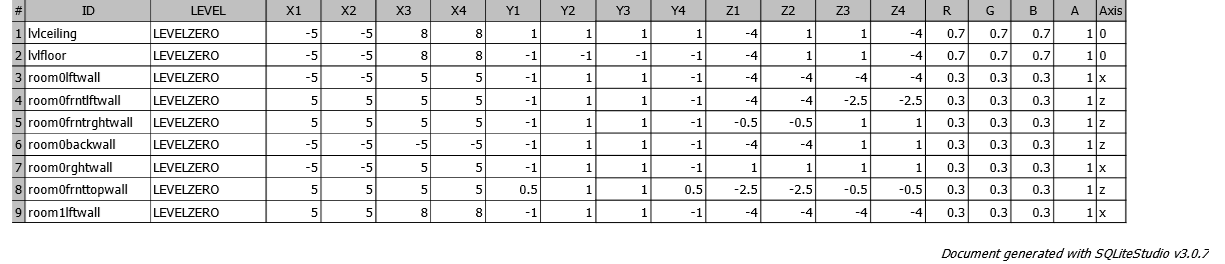
\includegraphics[width=18cm]{WALLS}

\subsubsection{Doors}

\subsubsection{Switches}
	 	 				
\subsection{Scripts}
 
\subsection{Images}
 
\subsection{Music}
	 	 	 				
\subsection{Sounds}
	 	 	 				

\end{document}